\section{Grasping}

\subsection{Gripper \& Forward Kinematics}

\begin{center}
\begin{figure}[H]
\centering
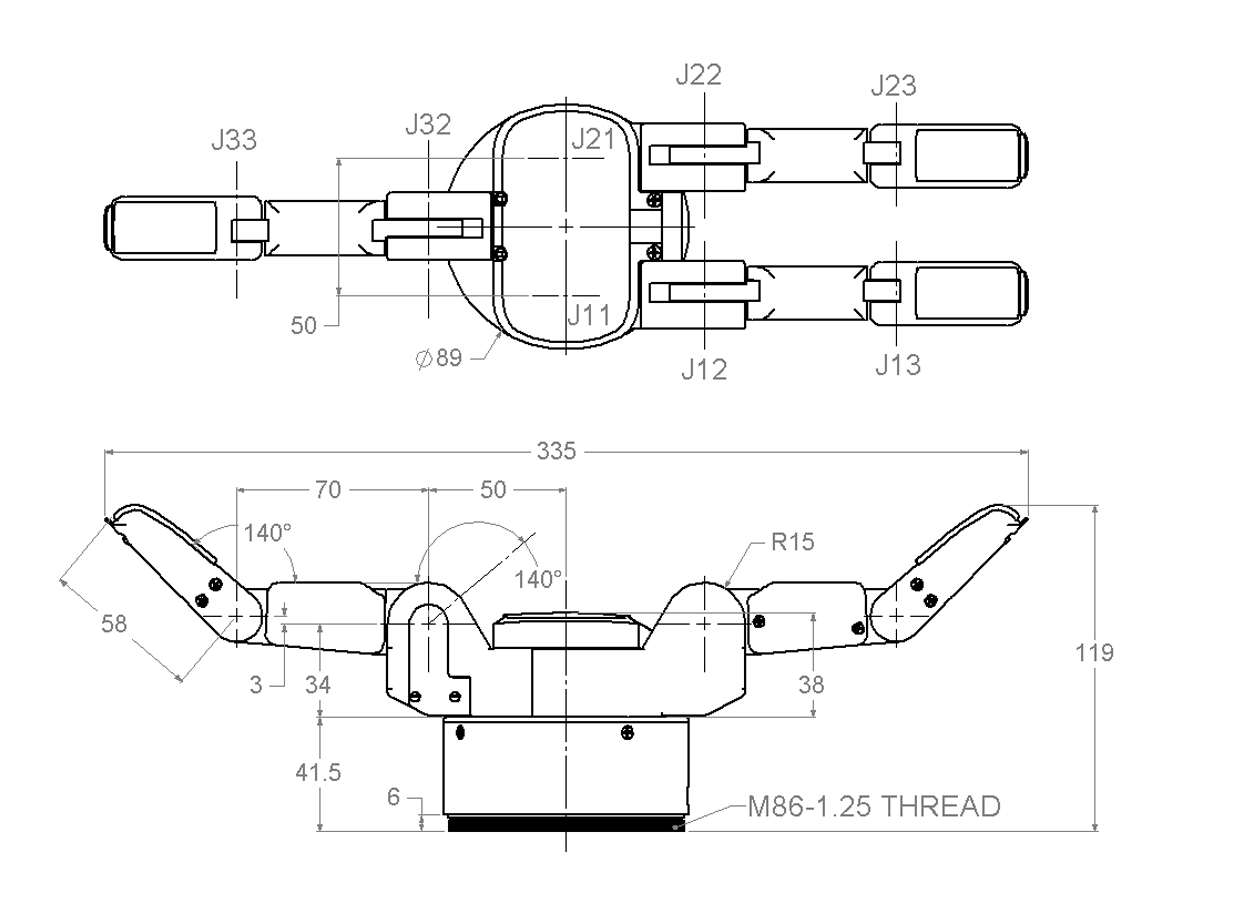
\includegraphics[width=12cm]{images/bh8-282-dimensions.png}\\[1cm]
\caption{Barrett Hand gripper (model BH8-282) dimensions}
\end{figure}
\end{center}


\subsection{Gripper Inverse Kinematics}

The following Inverse Kinematics analysis referes to one finger of the Barrett Hand gripper, which has 3 revolute joints. Finger 3 has only 2 
revolute joints for which the angle solutions are the same with the solutions of the last 2 joints of the other fingers. Let

\[
\mathbf{p} = \begin{bmatrix} p_x \\ p_y \\ p_z \\ \end{bmatrix}
\]

be the position of the grasp point for one finger. The first angle can easily be calculated as

\begin{equation}
φ_1 = atan2 \left( p_y, p_x \right)
\end{equation}

Next, we calculate the third angle based on the law of cosines (see fig.)
\[
cos \left( π - φ_3 - \frac{π}{4} \right) = \frac{L_2^2 + L_3^2 - p^2}{2 L_2 L_3}
\]
\[
cos \left(φ_3 + \frac{π}{4} \right) = \frac{p^2 - L_2^2 - L_3^2}{2 L_2 L_3}
\]
\begin{equation}
φ_3 = atan2 \left[ \pm \sqrt{1 - \left( \frac{p^2 - L_2^2 - L_3^2}{2 L_2 L_3} \right)^2} , \frac{p^2 - L_2^2 - L_3^2}{2 L_2 L_3} \right] - \frac{π}{4}
\end{equation}

After having calculated $φ_3$ we can calculate $φ_2 $

\[
tan \left( ψ + φ_2 \right) = \frac{p_z}{\sqrt{p_x^2 + p_y^2}}
\]
\[
tan \left( ψ \right) = \frac{L_3 sin \left( φ_3 + \frac{π}{4} \right) }{L_2 + L_3 cos \left( φ_3 + \frac{π}{4} \right)}
\]

\begin{equation}
φ_2 = atan2 \left( pz, \sqrt{p_x^2 + p_y^2} \right) - atan2 \left[ L_3 sin \left( φ_3 + \frac{π}{4} \right), L_2 + L_3 cos \left( φ_3 + \frac{π}{4} \right) \right]
\end{equation}

\subsection{Force closure}
The planar case, the spatial case \& convex hull test.

\subsection{Firm grasping algorithm \& Force control}